\chapter{Concepts and State of the Art}\label{ch:2}

\epigraph{The problem with object-oriented languages is they've got all this
implicit environment that they carry around with them. You wanted a banana but what you got was a gorilla holding the banana and the entire jungle.}{Joe Armstrong}

In this section we will discuss the most important concepts that are going to
be used in this thesis.


\section{Fundamental Concepts}

\subsection{Modeling, Metamodeling}\label{ch:2.1.1}

	Object-oriented programming is a paradigm which appeared in the
early '60 \cite{wiki:oop} and is based on the concept of defining object and
relationships between them. With the rapid growth of software system
object-oriented design has become a non-trivial problem even for small systems.
Thus the need of tools that can assist us in analyzing our design. 

	Modeling, as defined in the dictionary \cite{dictionary:modeling}, is the
representation, often mathematical, of a process, concept, or operation of a system, 
often implemented by a computer program.  There is no general accepted
definition for this term, but for the purpose of this thesis we can see a model
as a simplified version of a reality. As there can be many types of maps for the
same territory depending on the purpose (riding a bike, traveling to cities,
sightseeing) there can also be many types of models for the same system depending from which angle
we want view the system. Figure \ref{fig:CatModel} illustrates the idea.

\begin{figure}
\centering
\scalebox{0.4}{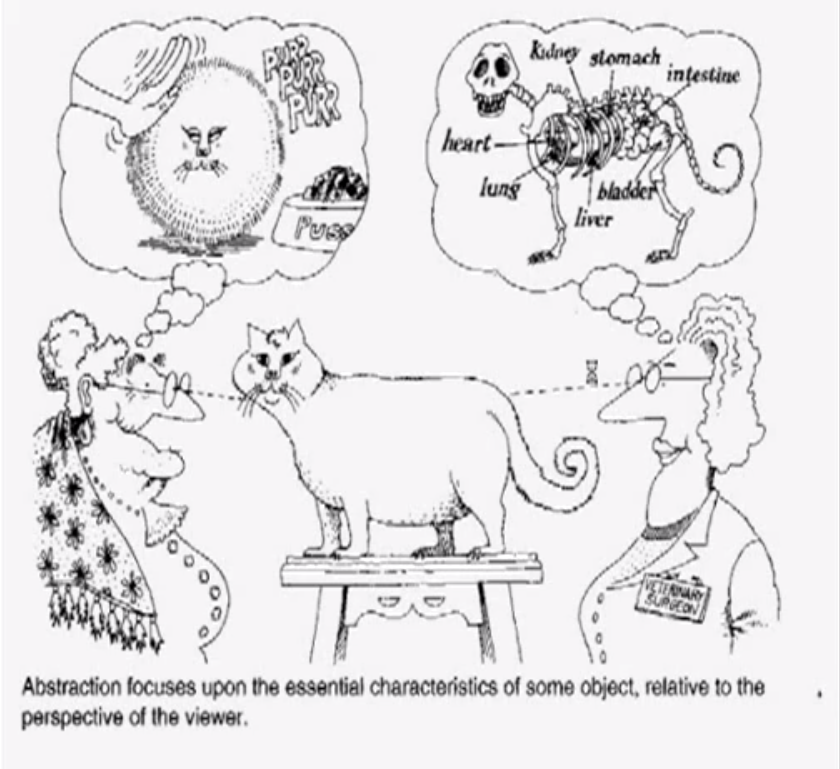
\includegraphics{../img/concepts/CatModel.png}}
\caption{The same cat but from different perspectives \cite{figure:CatModel}
\label{fig:CatModel}}
\end{figure}	

	
	In order to be able to work with models, software analysis tools need to be
able to understand and represent them, thus the need a way to describe models. For
this the concept of metamodeling has been introduced. The prefix meta- indicates 
an abstraction of a concept \cite{wiki:meta}. Formally, metamodel is an abstract 
syntax which governs the representation of a class of models. One of the most
common metamodels used in object oriented design (modeling) is UML
\cite{book:UMLDistilled}. One is able to describe its object oriented system by
simply showing the most important entities, i.e objects, and how
they interact with each other. In  figure \ref{fig:umlMetamodel} we have
representation of the XML metamodel described using UML.

   \begin{figure}
		\centering
		\scalebox{0.7}{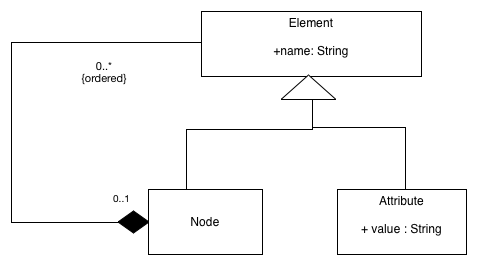
\includegraphics{../img/concepts/umlMetamodel.png}}
		\caption{XML metamodel\label{fig:umlMetamodel}}
	\end{figure}

	A very common case with tools is that people want them aggregated in one larger
tool. In order to do this we will need to define a way to describe software
analysis tools. As software analysis tools use metamodels for describing models,
it is natural to assume that we will need a meta-metamodel in order to describe
a metamodel. Thus a metamodel is also governed by a strict set of rules that form
a meta-metamodel. One can easily see that the definition is recursive and we
could continue with it indefinitely. In time many meta-metamodels have been
implemented in order to solve different problems (e.g Ecore, GME, KM3, \ldots{}
etc). For the purpose of this application we have used a simple
meta-metamodel\cite{thesis:CristianCaloghera} based on three elements: 
	\begin{itemize}
		\item Entity --- represents a generalization of a package, type, method, 
field \ldots{} etc
 
		\item Property --- represents a general characteristic computer for an entity
		\item Groups --- represents a tuple of one or more entities that are connected
by a relation (e.g inheritance, composition, generalization, all elements of an
entity, \ldots{} etc)
	\end{itemize}
	
	The figure \ref{fig:metamodel} represents the relationship between model,
meta-model, and so on.
	 

\begin{figure}
\centering
\scalebox{0.5}{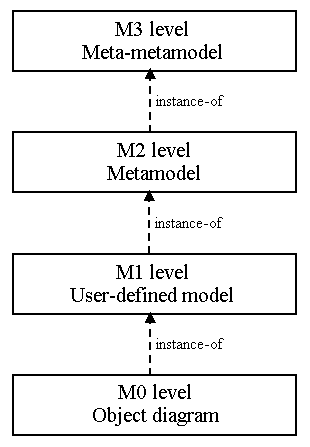
\includegraphics{../img/concepts/metamodel.png}}
\caption{Models and Metamodels\label{fig:metamodel}}
\end{figure}

\subsection{Ecliplse plugin}
	
	In computing, a plugin is a software component that adds a specific feature to an existing software application. 
When an application supports plugins, it enables customization. The best software analogy compares a plugin to an object in object-oriented
programming. A plugin, just like an object, encapsulates  the behavior and/or
data with which it can interacts with other plug-ins to form a running program.
	Eclipse is an extremely popular Java Integrated Development Environment (IDE)
and a strong competitor to NetBeans/SunOne Studio, JBuilder, and IntelliJ IDEA.
	Eclipse is made of a small core, with many plugins layered on top. Some plugins are nothing more than libraries that other plugins can use.
The base libraries used by all plugins are:

	\begin{description}[labelindent=2cm]
	\item[The Standard Widget Toolkit (SWT)]{Graphical components used everywhere
in Eclipse.}
	\item[The Plugin Developer Environment (PDE)]{ Classes that help us with the
plugin data manipulation, extensions, build process, and wizards.}
	\item[The Java Developer Toolkit (JDT)] {Classes used to programmatically
manipulate Java code.}
	\end{description}
	
	An Eclipse plugin has a set of main configuration files. These files 
define the APIs which will be used in our plugin and the dependencies to other
plugins.
	\begin{description}[labelindent=2cm]
		\item[MANIFEST.MF] - contains the OSGi configuration information.
		\item[plugin.xml] - optional configuration file, contains information about
Eclipse extensions.
	\end{description}
	An Eclipse plugin defines its metadata, like its unique identifier, its
exported API and its dependencies via the MANIFEST.MF file.
The plugin.xml file provides the possibility to create and contribute to Eclipse specific API. 
You can add extension points and extensions in this file.
Extension-points define interfaces for other plug-ins to contribute functionality. 
Functionality can be code and non-code based. For example a plug-in might
contain help content.
	

	In figure \ref{fig:eclipsePlugin} you can see an example of a development
process for a plugin.

\begin{figure}[h]
\centering
\scalebox{0.7}{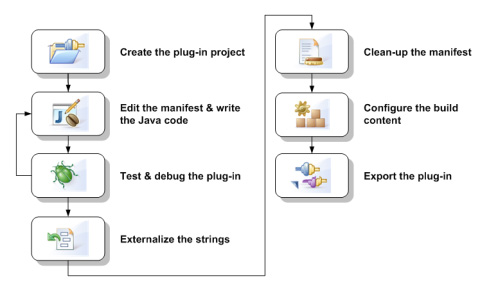
\includegraphics{../img/concepts/eclipsePlugin.jpg}}
\caption{Eclipse Plugin Development \cite{figure:eclipsePlugin}}
\label{fig:eclipsePlugin}
\end{figure}	

\subsection{Java Metadata}\label{ch:2.1.2}

	
	As mentioned above a model is nothing more or less than a simplified version of
a reality/system. In case of software analysis tools this system is actually a
program. In order to be able to manipulate programs (models) we need specific
language support for this type of programming, also called metaprogramming
\cite{website:metaprogramming}. 

	Many languages have different ways and levels of supporting metaprogramming.
In C++ this is done by using the template system (template metaprogramming), in
Java this is done by using the reflection API provided by the compiler and/or by using the annotation
language feature which allows metadata processing, i.e the ability to add
information to your code so that it can be used later for generating boiler
plate code or by enforcing constraints that can be verified at compile-time or
run-time. \cite{book:ThinkingInJava} 
	
	The syntax for defining an annotation is quite straight forward and resembles
very mucth the definition of an interface. The keyword used is \code{interface}
prefixed with the 'at' (@) sign. Different properties can be defined inside the annotation. If you set a default
value for the property it becomes optional. The type of a property can be 
primitive types, \code{Class<?>}, enum types or String.
	
	E.g:
	\small
	\begin{lstlisting}[language=Java,numbers=left]
@Retention(RetentionPolicy.SOURCE)
public @interface CreateWarning {
	String[] warning() default "Something is fishy"; 
}
	\end{lstlisting}
	\normalsize{}
	
	Usage:
	
	
	\small
	\begin{lstlisting}[language=Java,numbers=left]
Set<String> names = new HashSet<>();
....
//this message will be outputted as a warning
@CreateWarning("unsafe cast, must change")
String[] nameArray = (String[])names.toArray();
	\end{lstlisting}
	\normalsize{}
	
	\small
	\begin{lstlisting}[language=Java,numbers=left]
//the default message, will be outputted
@CreateWarning
public boolean equals(Object x) {
...
}
	\end{lstlisting}
	\normalsize{}
	
	Of course, as we love recursion, we have meta-annotations which
allow us to describe important information regarding annotations such as:
	\begin{itemize}
	 	\item what king of elements can the current annotation annotate
	 	\item how to store the information it provides ? (in the source file, in the
class file, just drop it after compilation, \ldots{} etc)
	 	\item if it can be repeated more than one time on the same element
	 	\item if the element is  documented
	\end{itemize}
	An example of such an annotation is provided in the definition of
\code{@CreateWarning}, i.e \code{@Retention}.
	
	The most common annotations that are used in {J}ava are:
	\begin{enumerate}
	  \item \textbf{@Override} -- indicates that the current method is an \\
 (re)implementation of method from the base class.
  
	  \item \textbf{@Deprecated} -- usually used in frameworks and indicates that
	  the entity will be removed in feature updates and support for it is no longer
 provided.
 
	  \item \textbf{@SuppressWarnings} -- stop the compiler from adding annoying
 warning.
	\end{enumerate}	

	The most complex part comes when we want to associate some semantics 
to our annotations. This is usually done by defining an 
\textbf{annotation processor}, i.e a compiler plugin which will be invoked when
our annotation(s) have been discovered by the compiler. After each 
annotation processor has finished some extra source code might have been
generated or some annotations might have been expanded in other annotations or both, in 
this case the compiler starts processing the code and invoking the annotation
processors again as can be seen in figure \ref{fig:annProc}.
	 In order to define an annotation processor one most create a class that
inherits from \code{javax.annotation.processing.AbstractProcessor}. The
most important function is \code{process(Set<TypeElement> annotations,
RoundEnvironment roundEnv)}, here you write your code for scanning, evaluating 
and processing annotations and generating java files. With RoundEnviroment passed 
as parameter you can query for elements annotated with a certain annotation.
	
\begin{figure}
\centering
\scalebox{0.8}{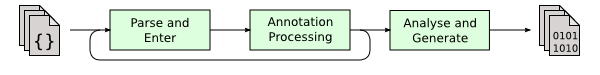
\includegraphics{../img/concepts/javac-flow.png}}
\caption{The compiler process with annotation
processing\cite{figure:javac-flow}\label{fig:annProc}}
\end{figure}

\subsection{Mirror API}
	Object-oriented languages traditionally support metalevel operations such as
reflection by reifying program elements such as classes, methods, fields,
packages, annotations \ldots{} etc, into objects that support reflective
operations such as getSuperclass or getMethods.
	In a typical object oriented language with reflection, (e.g., Java, C\#,
Scala, PHP, \ldots{} etc) one might query an instance for its class, as
indicated in the pseudo-code below:
\small
\begin{lstlisting}[language=Java,numbers=left]
class TreeMap {...}
TreeMap myTreeMap = new TreeMap();
Class<TreeMap> theTreeMapClass = myTreeMap.getClass();
\end{lstlisting}
\normalsize{}

	Another approach is introducing code on the fly, modifying the program as they
are executed. This is used in many scripting languages and goes by the name of
monkey patching or duck punching. Allows the user to locally modify the code of
class or elements that was already defined. \\
	One other approach would be the use of mirrors.
Mirrors have been used in class based systems such as Strongtalk, and even in
the Java world. The reflective operations are separated into distinct objects
called mirrors. Reflection is no longer tied into the behavior of every object.
Instead, it resides in separable components that can be removed or replaced. 
Reflection is now a distinct capability, in the sense of the object capability model.
	The most important thing to understand about mirrors is that they decouple the
reflection API from the standard object API, so instead of obj.getClass() you use reflect(obj). 
It's a seemingly small difference, but it gives you a few nice things:
	\begin{itemize}
		\item The object API isn't polluted, and there is no danger of breaking
reflection by overriding a reflective method.
		\item You can potentially have different mirror systems. Say, one that doesn't
allow access to private methods. This could end up being very useful for tools.
		\item The mirror system doesn't have to be included. If mirrors aren't used then there's no out-of-band to access code and 
pruning becomes viable.
Mirrors can be made to work on remote code, not just local code, since you don't need the reflected object to be in the same Isolate or VM as the mirror.	
	\end{itemize}

\section{Tools: CodePro}\label{ch:2.2}

	Software analysis tools are usually used by developers when something went
wrong or when someone wants to validate an idea. The developer will be running
the analysis tool(s) to compute complex metrics and interpreting the abstract numbers 
that the tool outputted and will try, in case of abnormal values, to find the
problem and propose a solution for it. The entire process is a pain kill and
mostly likely comes in the most inappropriate moment. \cite{tools:inCode}.

\begin{figure}[h]
\centering
\scalebox{0.5}{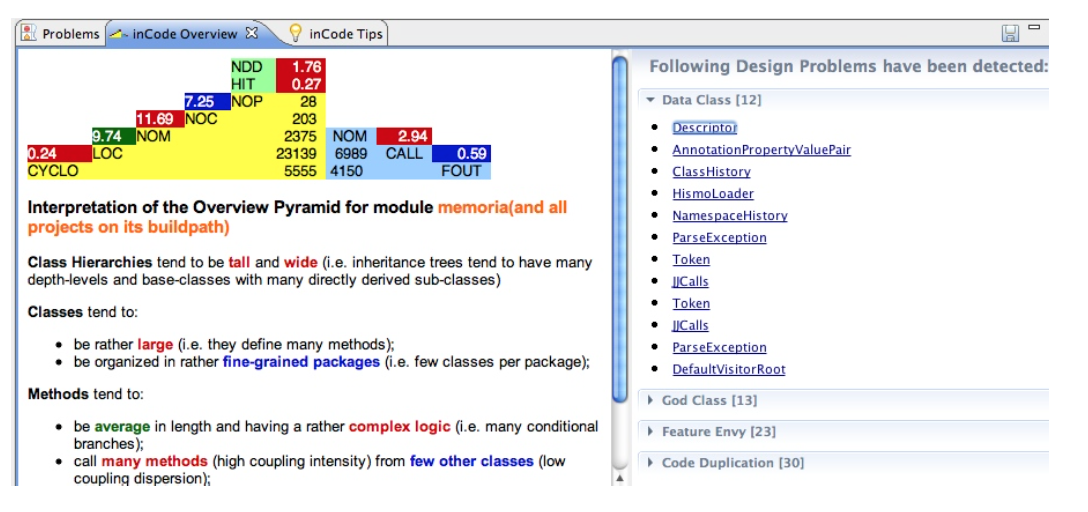
\includegraphics{../img/concepts/inCodeOverview.png}}
\caption{inCode overview \cite{tools:inCode} \label{fig:inCodeOverview}}
\end{figure}

	CodePro, or by its comercial name INCODE \cite{site:inCode}, is an eclipse
plugin which plans to solve this shortcomings of analysis tools by providing
continuous analysis of the code, marking problems solved and detecting new ones,
also providing arguments and tips on why was the problem detected, what causes
it and how it can be solved. In Figures \ref{fig:inCodeTips} and
\ref{fig:inCodeOverview} you can see examples of the features mentioned above.

\begin{figure}
\centering
\scalebox{0.4}{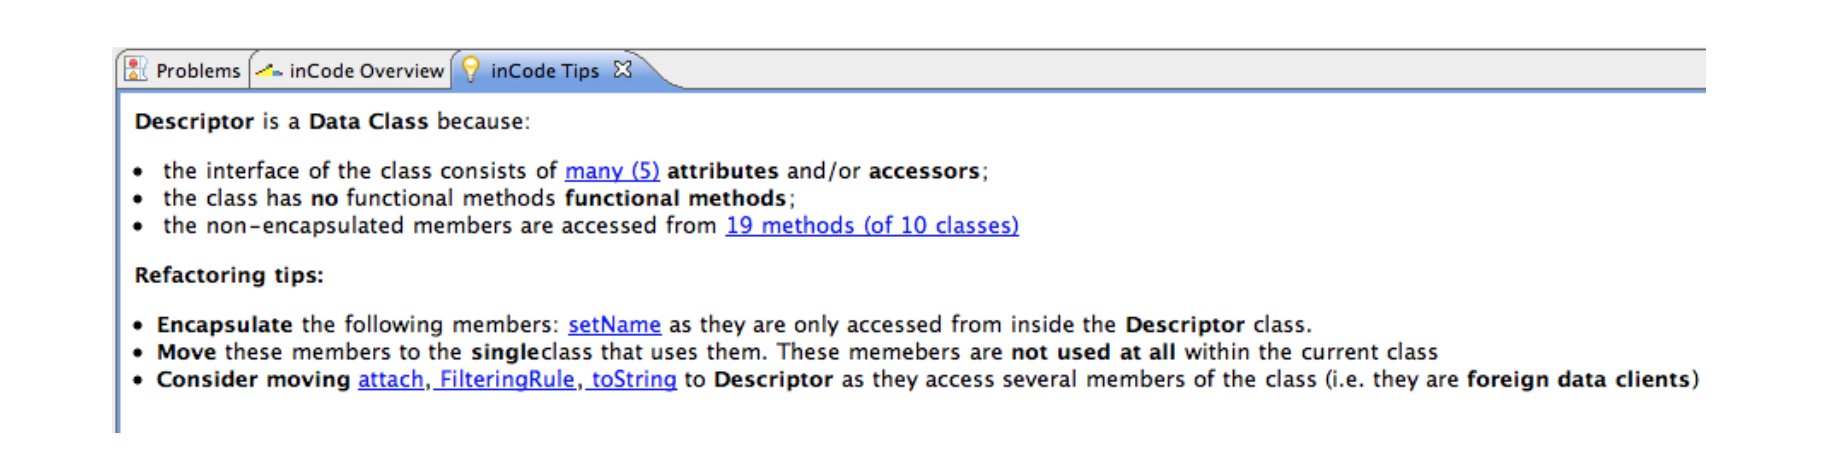
\includegraphics{../img/concepts/inCodeTips.png}}
\caption{inCode tips \cite{tools:inCode} \label{fig:inCodeTips}}
\end{figure}


	From an architectural point of view CodePro defines its own meta-metamodel 
,very similar to the one presented in \ref{ch:2.1.1}, but more complex. The
metamodel which is used is the one provided by Eclipse JDT library, wrapped to fit the
meta-metamodel defined. In \ref{fig:codeProUML} you can see an overview of the
general architecture. From analyzing the diagram we can spot some architectural 
problems related to type safety such as:
	\begin{itemize}
	  \item Consider the following code snippet: \code{aSystem.getGroup("class
	  group").applyFilter("model \\ class");}. We are using strings in order to
	  identify different metrics, types, filters \ldots{} etc.  
	  What will happen when someone changes the name of the entity ? What if we write Class instead of class ? \\
	 
	  \item property computers accept abstract entities instead of specific 
elements for which the computers are defined. The semantics definition is not 
preserved. If we use the Cyclomatic Complexity metric on a class or package  
instead of a method ? What is the expected return type since there is no
Cyclomnatic Complexity defined for them?\\
\code{public ResultEntity compute(AbstractEntityInterface anEntity)}

	\end{itemize}
	The tool that we have created is aimed at solving this shortcoming by providing
a way in which you can define a meta-metamodel and it will generate, based on
the provided meta-metadata, a concrete metamodel, everything becomes statically
typed.

\begin{figure}
\centering
\scalebox{0.55}{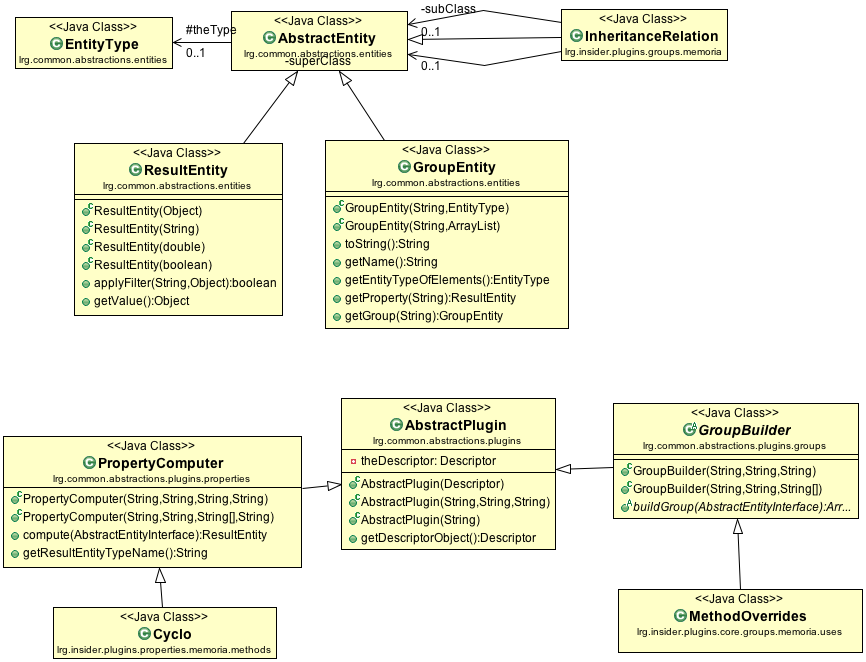
\includegraphics[angle=90]{../img/concepts/codeProUML.png}}
\caption{CodePro meta-metamodel and meta-model overview}
\label{fig:codeProUML}
\end{figure}

